\documentclass{article}
\usepackage{amsmath}
\usepackage{amssymb}
\usepackage{graphicx}
\usepackage{hyperref}
\usepackage[version=4]{mhchem}

\title{Problem 4}
\date{}

\begin{document}
\maketitle

\section*{Problem}
The area of trapezoid \(A B C D\) is \(318 \mathrm{~cm}^{2}\). The altitude is \(12 \mathrm{~cm}, A B\) is 13 cm , and \(C D\) is 37 cm . What is \(B C\), in centimeters?\\
(A) \(9 / 2\)\\
(B) \(10 / 3\)\\
(C) 6\\
(D) \(15 / 2\)\\
(E) \(13 / 2\)\\
\centering
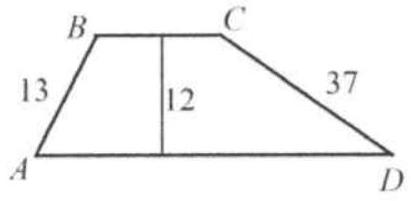
\includegraphics[width=\textwidth]{images/088.jpg}

\section*{Solution}
Solution not available.

\end{document}
